\documentclass{lab}

\usepackage{graphicx}
\usepackage{float}

\title{ENGG1003 - Lab 1}
\author{Brenton Schulz}
\date{\today}

\begin{document}
\maketitle

\section{Introduction}
This laboratory exposes you to the fundamental tools required to write computer programs in C. No prior programming experience is assumed

\section{C Programming Basics}
In order to write programs in C (and most other languages) the following software tools are required:

\begin{itemize}
\item An \textit{editor}, to create and edit raw text files.
\item A \textit{compiler}, to convert your text files into an \textit{executable} file.
\end{itemize}

A programming editor is very different to a \textit{word processor} (eg: Microsoft Word) in that it displays and stores raw ASCII text only. What you see printed to the screen represents the \textit{actual data} stored in the file. By contrast, Word will store a combination of text and display formatting and, as such, is not suitable for writing code.

Programming editors will generally have features optimised for coding, such as:

\begin{itemize}
\item Syntax highlighting
\item Line numbering
\item Auto completion
\item Pre-emptive error notifications
\item Communication with the compiler to highlight errors
\item Automatic indenting
\item Highlighting of matching blocks 
	\begin{itemize}
		\item ie: an easy method to find matching pairs of ( ), \{ \}, " ", etc.
	\end{itemize}
\end{itemize}

It is hoped that you will discover these features and learn to work with them. In time you will learn which features work well with your style and which simply get in the way.

For the time being the ``compiler'' noun will be used to colloquially reference a highly complex set of software tools which turn your source code into an executable binary file. You will be shielded from the details until otherwise necessary.

\subsection{Introduction to OnlineGDB}

OnlineGDB is a basic (\textit{very} basic) browser-based development environment for a variety of programming languages. It gives you access to an editor, a small amount of cloud storage, compiler, and standard input~/~output. It also contains a \textit{debugging} feature however for technical reasons\footnote{It only allows one debug session per IP address. The entire campus uses the same public IP so we can't use it in labs.} we won't be using it.

All compilation and execution is performed on the OnlineGDB server. As such, the service has an incredibly low barrier to entry: there is (almost) zero installation/configuration required to get started running code.

\textbf{Task:} Open a web browser and navigate to \url{http://www.onlinegdb.com}.\\ \\ \textbf{NB:} If a demonstrator sees you using Edge or IE they may instinctively think you need more help than students using Chrome or Firefox.

\begin{figure}[H]
\begin{center}
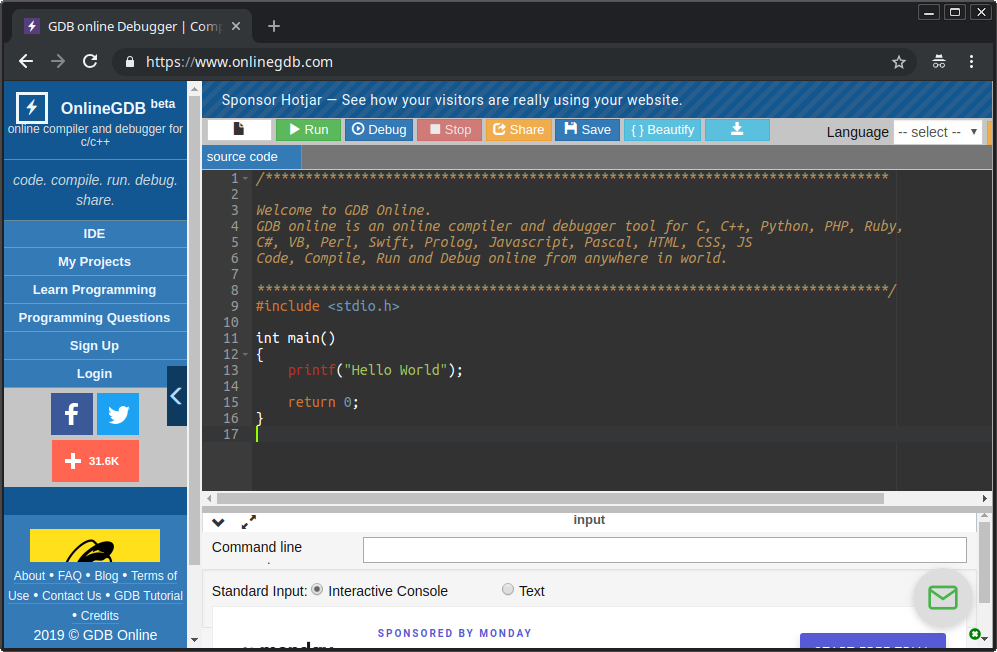
\includegraphics[width=\textwidth]{onlinegdb.png}
\end{center}
\caption{The view when OnlineGDB is first opened.}\label{fig:onlinegdb}
\end{figure}

After OnlineGDB has loaded you will be greeted with the screen seen in Figure \ref{fig:onlinegdb}. The large area in the middle is the editor screen, this is where you will type C code. Immediately you can observe that this editor supports line numbering and syntax highlighting.

Above the editor is a toolbar which, from left to right, performs the following functions:

\begin{enumerate}
\item Create a blank new file
\item Run the project
\item Debug the project (not used in ENGG1003)
\item Stop execution of a running program
\item Share - Generates a link to your current source code
\item Save - When logged in this saves the project files to your personal cloud storage
\item \{ \} Beautify - Modifies your code's whitespace to adhere to the OnlineGDB indenting style (NB: I tried this at time of writing and it didn't work on my personal computer. Go figure.)
\item Download - Downloads the currently viewed file.
\end{enumerate}

The area below the editor is where standard output is written to and standard input read from. When the code is run its appearance changes to that of a basic console (ie: the GUI elements disappear and it becomes just text).

\textbf{Task:} Configure OnlineGDB to run C code by selecting ``C'' from the ``Language'' drop-down box in the upper-right. This website supports many languages\footnote{MATLAB is not one of them because it is a \textit{very} expensive commercial package} so feel free to come back here later if you're interested in learning any of the others. Python, although not taught in an Engineering degree, is a common choice for Engineering PhD students as a free MATLAB alternative and is probably worth playing around with.

\textbf{Task:} Click the green Run button. The box at the bottom of the screen will produce a ``Compiling'' animation and, after execution of the template code, will produce the output seen in Figure \ref{fig:onlinegdb_hello}.

\begin{figure}[H]
\begin{center}
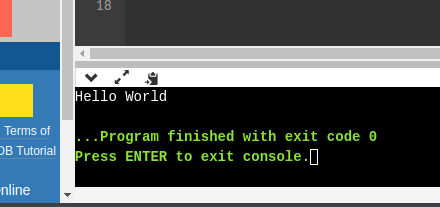
\includegraphics[width=0.7\textwidth]{onlinegdb_hello.png}
\end{center}
\caption{A cropped screenshot showing the "Hello World" program output.}\label{fig:onlinegdb_hello}
\end{figure}

\textbf{Off-topic note:} Remember the ``returns zero to the operating system'' comment in lecture 1? Well that's what the text ``...Program finished with exit code 0'' is referencing. The 0 is the number that \texttt{main()} \textit{returned}. We will learn about \textit{function return values} later in the semester.

\textbf{Tasks:} 

\begin{enumerate}

\item Running the default template demonstrates \textit{standard output}, modify the code to match that in Listing~\ref{lst:stdio}. While making the changes you will observe OnlineGDB's auto-complete features. When, for example, you type a double quote " character it \textit{automatically} types two and places the cursor between them. It will also provide auto-complete suggestions, although many of them will be inappropriate (it is, after all, just a computer program; not a science fiction grade artificial intelligence).

What other ``helpful'' editor behaviour did you notice? Some of it will be annoying at first (some of it will be annoying \textit{forever}) but learning to work with the editor's features will improve your coding speed in the long term.

\begin{lstlisting}[style=CStyle,caption=A basic C program which demonstrates input and output.,label=lst:stdio]
#include <stdio.h>

int main() {
	int k;
	scanf("%d", &k);
	printf("You entered: %d\n", k);
	return 0;
}
\end{lstlisting}

\item After editing the code press Run. After it is compiled you will notice that the console is just displaying a cursor. This is because \texttt{scanf()} waits for data to be typed (specifically, it will wait until a new line character, ASCII value 10, is sent).

\item Type an integer and press \texttt{enter / return}. There will be some ``lag'' because the data is being sent to OnlineGDB's server before being displayed.

\item After pressing enter the console should display the text ``\texttt{You typed: 123}''.

\item Run the program again except this time don't type just an integer, try typing a word, or a word containing a number, or a number followed by letters (with and without a space). What is the behaviour each time? Are you getting annoyed by the slow compile time and lag yet? OnlineGDB may be simple but it is, at times, a compromise.

\end{enumerate}

\section{Git}
\subsection{What on Earth is git?}

\section{Getting started with C in Ubuntu Linux}

Linux is not supported by university IT but, personally, I find it to be a fantastic development platform. The following instructions are completely optional, only do this if you are keen to learn.

Installing Ubuntu is beyond the scope of this document (and course). If you think this is a daunting task I would recommend only using the officially supported tools to complete ENGG1003. There are many thousands of websites and YouTube videos which will guide you through the Ubuntu (or Mint, Arch, etc.) installation process. \textbf{NB:} Installing a new operating system can \textit{very easily} destroy all existing software on a machine. Don't do this if you don't know what you're doing.

That out of the way, here's how you can get started. These steps assume a fresh Ubuntu 18.04 installation, in other distributions YMMV\footnote{Your mileage may vary. ie: this steps might not work}:

\begin{enumerate}
\item The C compiler in Linux (and OnlineGDB, and \textit{many} other platforms) is gcc (the GNU C Compiler). To install it, open a terminal (\texttt{ctrl + alt + t}) and type:

\texttt{\$ sudo apt install gcc libc6-dev gedit}\\ (the \$ indicates the terminal prompt, don't type that character)

When prompted, enter your password, wait a few seconds, press \texttt{enter} if it wants installation confirmation, and wait a few more seconds. An Internet connection is required for apt to download the required software.

The \texttt{libc6-dev} package provides all the basic C libraries (\texttt{printf} etc.) and \texttt{gedit} is a basic text editor.

\item Lets make a new directory for writing C files, type:
\begin{enumerate}
	\item \texttt{\$ mkdir c}
	\item \texttt{\$ cd c}
\end{enumerate}
The first command creates a directory called ``c'' and the second ``changes into'' that directory.

\item Create a new .c file. We will do this in \texttt{gedit} (because it is easy and simple) but there are many others (the more nerdy among you may want to learn \texttt{vim} or \texttt{emacs}. They are \textit{very} powerful editors).

Type: \texttt{\$ nohup gedit test.c \&} \\ (The \& symbol at the end of a command runs the command ``in the background''. This gives you the command line back straight away, instead of having to quit gedit first. Preceding the command with \texttt{nohup} stops \texttt{gedit} from closing if you close the terminal window)

\item Type out the code seen in Figure \ref{fig:gedit}.

\item Click the Save button (or type \texttt{ctrl + s}).

\begin{figure}[H]
\begin{center}
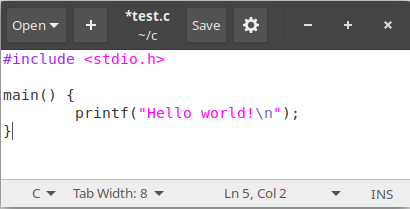
\includegraphics[width=0.5\textwidth]{gedit.png}
\end{center}
\caption{The gedit window with some C code typed out.}\label{fig:gedit}
\end{figure}

\item Move the \textit{keyboard focus} back to the terminal (ie: click the terminal window).

\item If you can see the command prompt yet, press \texttt{enter}

\item You can type \texttt{ls} to see a list of all files in the current directory. \texttt{test.c} should be there.

\item To compile the \texttt{.c} file run: \texttt{\$ gcc test.c -o test}

This will create a binary executable called \texttt{test}. If the \texttt{-o} \textit{command line argument} is not given \texttt{gcc} the binary file defaults to the name \texttt{a.out}.

\item Run \texttt{test} by typing: \texttt{\$ ./hello}

The \texttt{./} is a special character string meaning ``relative to the current directory''. If you try to run \texttt{test} from any other directory nothing will happen because \texttt{test} is a built-in command. With most other names you will get a ``Command not found...'' error.

\item When the program runs you should see something similar to Figure \ref{fig:c_ubuntu}.

\item Go back to \texttt{gedit} and keep coding as you desire. Return to the command line to run \texttt{gcc} to re-compile your code. \textbf{NB:} The command line has a \textit{history} feature, pressing the up arrow will scroll through past commands, \textit{you don't need to type them out from scratch}.

\item If you enjoyed this you're a bit weird, welcome to the club! Recommended further reading would be a tutorial on \texttt{make} followed by investigations into more powerful editors like \texttt{vim}.

\begin{figure}[H]
\begin{center}
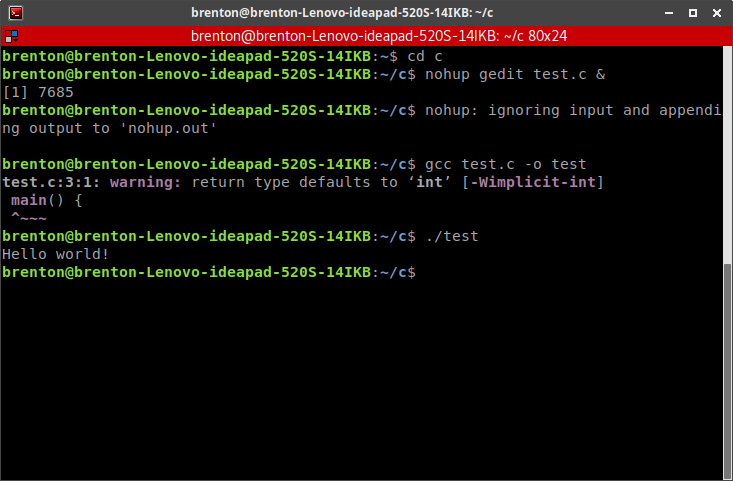
\includegraphics[width=0.8\textwidth]{c_ubuntu.png}
\end{center}
\caption{The complete command line sequence performed in these steps.}\label{fig:c_ubuntu}
\end{figure}


\end{enumerate}

\end{document}